\section{测度空间}
\label{sec:meas-measure-spaces}

上一节的两项要求针对两个不同的对象：一项限定哪些集合允许测量，另一项规定怎样给这些集合赋予大小。本节把它们分开建立。

我们先用$\sigma$代数描述允许测量的集合族，并在度量空间上由开集得到Borel集；再在其上定义可数可加的测度，推出比较集合与取极限的规则；最后讨论零测集，说明忽略哪些点不会改变测量，以及怎样把零测集的子集也纳入可测范围。

\subsection{$\sigma$代数}
\label{sec:meas-sigma-algebras}

\paragraph{能够区分哪些集合}
设$X=\{1,2,3,4\}$。若允许测量全部$16$个子集，就能单独询问每个点的大小。若我们只知道每个点属于$\{1,2\}$还是$\{3,4\}$，能够回答的就只有下面四个集合：
\[
 \varnothing,\quad\{1,2\},\quad\{3,4\},\quad X.
\]
单点$\{1\}$这时无法单独测量。两种集合族的底集相同，区分能力不同。

可以把一个集合族看成一份“允许提问的清单”：清单上的集合，才能问它有多大。无论清单选哪一份，都应满足上一节的封闭性要求：能问“在$A$中吗”，就能问“不在$A$中吗”；能问一列集合中的每一个，就能问“至少在其中一个中吗”。把这两条写下来，就是下面的定义。

\begin{definition}[$\sigma$代数]
\label{def:meas-sigma-algebra}
设$X$是集合，$\mathcal A$是$X$的一族子集。若
\begin{enumerate}
 \item $X\in\mathcal A$；
 \item $A\in\mathcal A$蕴含$X\setminus A\in\mathcal A$；
 \item $A_1,A_2,\dots\in\mathcal A$蕴含$\bigcup_{n\geq1}A_n\in\mathcal A$，
\end{enumerate}
则称$\mathcal A$为$X$上的一个\term{$\sigma$代数}（sigma-algebra），称$(X,\mathcal A)$为\term{可测空间}（measurable space），称$\mathcal A$中的集合为\term{可测集合}（measurable set）。
\end{definition}

定义只列出补集与可数并，其他运算由它们得到。由第1、2条，$\varnothing=X\setminus X\in\mathcal A$；在第3条中从某项起全取$\varnothing$，得到有限并封闭。可数交由De Morgan律化为补集与并：
\[
 \bigcap_{n\geq1}A_n=X\setminus\bigcup_{n\geq1}(X\setminus A_n).
\]

差集$A\setminus B=A\cap(X\setminus B)$也属于$\mathcal A$。所以从可测集合出发，经可数次补、并、交、差得到的集合仍然可测。开头的两种清单都满足这些条件：幂集$\mathcal P(X)$含全部子集；四个集合$\varnothing,\{1,2\},\{3,4\},X$中任一个的补集、任意几个的并也都在其中。

\paragraph{生成的$\sigma$代数}
实际问题中，我们通常只点名少数必须能测量的集合，例如区间或若干类别，希望由它们补齐其余集合。给定$X$的一族子集$\mathcal C$，包含$\mathcal C$的$\sigma$代数至少有幂集一个。令$\sigma(\mathcal C)$为所有包含$\mathcal C$的$\sigma$代数之交，称为$\mathcal C$\term{生成的$\sigma$代数}（generated sigma-algebra）。

这个交确实是$\sigma$代数：每个参与求交的$\sigma$代数都含$X$，并对补集、可数并封闭；交集中的元素同时属于它们全体，运算结果也同时属于它们全体。它包含$\mathcal C$，又包含于任何包含$\mathcal C$的$\sigma$代数，所以是其中最小的一个。

这与线性代数中“由一组向量张成的子空间”很像：张成的子空间是包含这组向量的最小子空间，也可以写成所有包含它们的子空间之交。那里的运算是线性组合，这里的运算是补集和可数并。不同之处在于，张成的子空间有“全体有限线性组合”这样的显式表达，而$\sigma(\mathcal C)$一般写不出这样的清单，只能用封闭性来描述。

\begin{example}[有限分组生成的$\sigma$代数]
\label{ex:meas-partition-sigma}
在$X=\{1,2,3,4\}$上取$\mathcal C=\{\{1\},\{2\}\}$。生成的$\sigma$代数必须含$\{1\}$、$\{2\}$，以及
\[
 X\setminus(\{1\}\cup\{2\})=\{3,4\}.
\]
于是它含分组$\{1\},\{2\},\{3,4\}$中任意几组的并，共$2^3=8$个集合。这$8$个集合对补集和并已经封闭，所以它们就是$\sigma(\mathcal C)$，而$\{3\}$不在其中。
\end{example}

图~\ref{fig:meas-partition-sigma}比较了三种分组。有限集合上的$\sigma$代数都由某个分组决定：可测集合恰是若干组之并，组分得越细，可以单独测量的集合就越多。

\begin{BookInlineFigure}
  \centering
  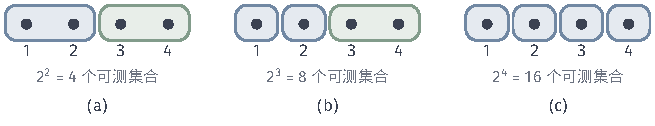
\includegraphics[width=110.938mm]{figures/04-spaces-measures-and-geometry/02-measure/tikz/meas-sigma-algebra-partition/figure.pdf}
  \caption{四点集合$X=\{1,2,3,4\}$上由分组生成的$\sigma$代数。每个色块是一组，可测集合恰是若干组之并。(a)分成$\{1,2\},\{3,4\}$两组；(b)分成$\{1\},\{2\},\{3,4\}$三组；(c)每点自成一组，得到全部子集。}
  \label{fig:meas-partition-sigma}
\end{BookInlineFigure}

生成操作补齐的只是可数运算的封闭性，未必得到所有希望测量的集合。在$\mathbb R$上取全体单点组成的族$\mathcal C$，令$\mathcal D$为可数集合与补集可数的集合的全体。

$\mathcal D$含$\mathbb R$，对补集封闭。对一列$\mathcal D$中的集合，若都可数，则并可数；若其中有一个补集可数，则并的补集包含于它的补集，也可数。所以$\mathcal D$是含全部单点的$\sigma$代数，于是$\sigma(\mathcal C)\subseteq\mathcal D$。

而$[0,1]$与它的补集都不可数，所以$[0,1]\notin\mathcal D$。可见单点生成的$\sigma$代数不含任何非退化区间；要测量区间，生成族里必须直接放入区间或开集。

\paragraph{Borel集}
在度量空间中已经有一族自然的集合：开集。第~\ref{chap:topological-spaces}章用开集表达连续、收敛与紧性，第~\ref{chap:metric-spaces}章又用开球刻画度量空间的开集。把开集作为生成族，得到的可测范围就与这些结构相容。

\begin{definition}[Borel $\sigma$代数]
\label{def:meas-borel}
设$X$是度量空间（更一般地，拓扑空间）。由全体开集生成的$\sigma$代数称为$X$的\term{Borel $\sigma$代数}（Borel sigma-algebra），记作$\mathcal B(X)$，其中的集合称为\term{Borel集}（Borel set）。
\end{definition}

开集的补集是闭集，所以闭集都是Borel集；可数个闭集的并、可数个开集的交也是Borel集。例如$\mathbb Q$是可数个闭集$\{q\}$的并，$[0,1)=\bigcap_{n\geq1}(-1/n,1)$是可数个开集的交，二者都是Borel集。

要强调的是，$\mathcal B(X)$只规定了哪些集合允许测量，并没有规定任何集合的大小。同一个Borel结构上可以放置长度、点质量或它们的组合等不同的测度。

\paragraph{实轴上的生成族}
直接处理全部开集并不方便。下面说明较小的区间族已经够用，关键是把任意开集写成可数个区间的并。

\begin{lemma}[开集的有理区间表示]
\label{lem:meas-open-rational-intervals}
$\mathbb R$中每个开集$U$都是有理端点开区间的可数并。
\end{lemma}

\begin{proof}
任取$x\in U$。因为$U$是开集，存在$r>0$使$(x-r,x+r)\subseteq U$。有理数在实轴上稠密，可取有理数$p,q$满足
\[
 x-r<p<x<q<x+r,
\]
于是$x\in(p,q)\subseteq U$。

所以$U$等于所有含于$U$的有理端点开区间$(p,q)$之并。这样的区间由有序对$(p,q)\in\mathbb Q\times\mathbb Q$确定，而$\mathbb Q\times\mathbb Q$可数，所以这是可数并。
\end{proof}

\begin{theorem}[$\mathcal B(\mathbb R)$的生成族]
\label{thm:meas-borel-generators}
下列每一族集合都生成$\mathcal B(\mathbb R)$：(1)全体开区间$(a,b)$；(2)全体半直线$(a,+\infty)$；(3)全体半直线$(-\infty,a]$；(4)全体左开右闭区间$(a,b]$。在(2)(3)中只取有理数$a$也够用。
\end{theorem}

\begin{proof}
各族中的集合都是开集、闭集或二者之交，属于$\mathcal B(\mathbb R)$，所以它们生成的$\sigma$代数都含于$\mathcal B(\mathbb R)$。反方向只需说明每个开集属于各族生成的$\sigma$代数。对族(1)，这就是引理~\ref{lem:meas-open-rational-intervals}。

其余各族都能经可数运算得到开区间。先看半直线。取有理数列$p_n$严格递减趋于$a$，则
\[
 (a,+\infty)=\bigcup_n(p_n,+\infty),
\]
所以有理端点的半直线已能生成族(2)。又因$(-\infty,a]$的补集是$(a,+\infty)$，族(3)与族(2)生成同一个$\sigma$代数。

再看半开区间与开区间。由下面两个等式：
\[
 (a,b]=(-\infty,b]\setminus(-\infty,a],\qquad
 (a,b)=\bigcup_{n}\,(a,\,b-1/n]
\]
（后式中$n$取使$b-1/n>a$的整数），可知开区间属于族(3)或族(4)生成的$\sigma$代数。
\end{proof}

同样的论证在$\mathbb R^d$中成立：每个开集是可数个有理顶点开矩形之并，所以开矩形生成$\mathcal B(\mathbb R^d)$；把开矩形写成左开右闭矩形的可数并，可知左开右闭矩形$\prod_i(a_i,b_i]$也生成$\mathcal B(\mathbb R^d)$。

\subsection{测度及其基本性质}
\label{sec:meas-measures}

\paragraph{测度的定义}
可测范围确定以后，要给每个可测集合配一个非负的大小，并要求可数可加。允许取值$+\infty$，因为整条实轴的长度、无限集合的元素个数都没有有限的值。在$[0,+\infty]$中约定$a+(+\infty)=+\infty$，非负项级数的和是部分和的上确界，可以为$+\infty$。

\begin{definition}[测度]
\label{def:meas-measure}
设$(X,\mathcal A)$是可测空间。映射$\mu:\mathcal A\to[0,+\infty]$若满足$\mu(\varnothing)=0$，并且对两两不交的$A_1,A_2,\dots\in\mathcal A$有
\begin{equation}
 \mu\Bigl(\bigcup_{n\geq1}A_n\Bigr)=\sum_{n\geq1}\mu(A_n),
 \label{eq:meas-countable-additivity}
\end{equation}
则称$\mu$为$(X,\mathcal A)$上的\term{测度}（measure），称$(X,\mathcal A,\mu)$为\term{测度空间}（measure space）。式~\eqref{eq:meas-countable-additivity}称为\term{可数可加性}（countable additivity）。
\end{definition}

非负项级数的和与求和次序无关，所以式~\eqref{eq:meas-countable-additivity}右端不依赖集合的排列方式，这与左端的并集不依赖排列相一致。条件$\mu(\varnothing)=0$排除了一切集合都取$+\infty$的平凡赋值；若某个$A$满足$\mu(A)<+\infty$，取$A_1=A$、其余为空集，由式~\eqref{eq:meas-countable-additivity}也能推出它。

\paragraph{计数测度与点质量}
在任意可测空间上，令$\mu(A)=\#A$（$A$为无限集时取$+\infty$），称为\term{计数测度}（counting measure）。核对可数可加性：若不交的$A_n$中只有有限个非空且都是有限集，两边都是元素总数；若某个$A_n$无限，或有无限多个$A_n$非空，并集无限，右边的级数也发散到$+\infty$。

固定$x\in X$，规定
\[
 \delta_x(A)=\begin{cases}1,&x\in A,\\0,&x\notin A,\end{cases}
\]
称为点$x$处的\term{Dirac测度}（Dirac measure）。不交集合列中至多一个含$x$，所以可数可加性成立。

这个定义只读取可测集合$A$是否含$x$，并不要求单点$\{x\}$本身可测。例如在$\mathcal A=\{\varnothing,\{1,2\},\{3,4\},X\}$上，$\delta_1$给$\{1,2\}$赋值$1$，给$\{3,4\}$赋值$0$，尽管$\{1\}$不可测。

把可数个点质量按非负权重相加，得到$\mu=\sum_kw_k\delta_{x_k}$，即$\mu(A)=\sum_{k:x_k\in A}w_k$。它推广了上一节的加权计数。核对可数可加性时要交换两重求和：
\[
 \sum_n\sum_kw_k\delta_{x_k}(A_n)=\sum_k\sum_nw_k\delta_{x_k}(A_n).
\]
非负二重级数的两种累次求和相等，因为任意有限部分和都不超过另一种次序的总和，令有限范围扩大即得两个方向的不等式。

例如在$\mathbb N=\{1,2,\dots\}$上取$\mu=\sum_n2^{-n}\delta_n$。总量是
\[
 \mu(\mathbb N)=\sum_{n\geq1}2^{-n}=1,
\]
偶数集的测度是
\[
 \mu(\{2,4,6,\dots\})=\sum_{m\geq1}2^{-2m}=\sum_{m\geq1}4^{-m}=\frac13.
\]

\paragraph{有限性条件}
测度可以整体取$+\infty$，但不同测度“无限”的方式差别很大，后面一些结论要区分它们。

\begin{definition}[有限测度、概率测度与$\sigma$有限测度]
\label{def:meas-finiteness}
设$(X,\mathcal A,\mu)$是测度空间。若$\mu(X)<+\infty$，称$\mu$为\term{有限测度}（finite measure）；若$\mu(X)=1$，称$\mu$为\term{概率测度}（probability measure）；若存在$X_1,X_2,\dots\in\mathcal A$使$X=\bigcup_nX_n$且每个$\mu(X_n)<+\infty$，称$\mu$为\term{$\sigma$有限测度}（sigma-finite measure）。
\end{definition}

有限测度都是$\sigma$有限的。$\mathbb N$上的计数测度总量为$+\infty$，但$\mathbb N=\bigcup_n\{n\}$且每个单点计数为$1$，所以它$\sigma$有限：整体无限，却能切成可数个有限的片。

$\mathbb R$上以全部子集为可测范围的计数测度不是$\sigma$有限的。若$\mathbb R=\bigcup_nX_n$且每个$X_n$都是有限集，$\mathbb R$就可数了，这是矛盾。唯一性定理和乘积测度需要$\sigma$有限条件，下面的基本性质不需要；我们在每处单独声明，不把它当作统一假设。

\paragraph{基本性质}
可数可加性只直接说到不交集合。比较有包含关系的集合、处理互相重叠的集合、对集合列取极限，都要先把集合拆成不交的部分。

\begin{theorem}[测度的基本性质]
\label{thm:meas-basic-properties}
设$(X,\mathcal A,\mu)$是测度空间，以下集合都属于$\mathcal A$。
\begin{enumerate}
 \item 有限可加性：若$A_1,\dots,A_m$两两不交，则
 \begin{equation}
  \mu\Bigl(\bigcup_{k=1}^mA_k\Bigr)=\sum_{k=1}^m\mu(A_k).
  \label{eq:meas-finite-additive}
 \end{equation}
 \item 单调性：$A\subseteq B$蕴含$\mu(A)\leq\mu(B)$；若还有$\mu(A)<+\infty$，则
 \begin{equation}
  \mu(B\setminus A)=\mu(B)-\mu(A).
  \label{eq:meas-monotone-difference}
 \end{equation}
 \item 可数次可加性：$A_n$不必两两不交，都有
 \begin{equation}
  \mu\Bigl(\bigcup_nA_n\Bigr)\leq\sum_n\mu(A_n).
  \label{eq:meas-countable-subadditive}
 \end{equation}
 \item 从下连续性：若$A_1\subseteq A_2\subseteq\cdots$，则
 \begin{equation}
  \mu\Bigl(\bigcup_nA_n\Bigr)=\lim_{n\to\infty}\mu(A_n).
  \label{eq:meas-continuity-below}
 \end{equation}
 \item 从上连续性：若$A_1\supseteq A_2\supseteq\cdots$且$\mu(A_1)<+\infty$，则
 \begin{equation}
  \mu\Bigl(\bigcap_nA_n\Bigr)=\lim_{n\to\infty}\mu(A_n).
  \label{eq:meas-continuity-above}
 \end{equation}
\end{enumerate}
\end{theorem}

\begin{proof}
第1条在可数可加性中令$A_n=\varnothing$（$n>m$）即得。

对第2条，$B=A\cup(B\setminus A)$是不交并，由第1条
\[
 \mu(B)=\mu(A)+\mu(B\setminus A)\geq\mu(A).
\]
当$\mu(A)$有限时，两边可以减去$\mu(A)$，得到差集的公式。

对第3条，先把重叠的部分去掉：令$B_1=A_1$，$B_n=A_n\setminus\bigcup_{k<n}A_k$。这些$B_n$两两不交，$B_n\subseteq A_n$，并且$\bigcup_nB_n=\bigcup_nA_n$。由可数可加性与单调性，
\[
 \mu\Bigl(\bigcup_nA_n\Bigr)=\sum_n\mu(B_n)\leq\sum_n\mu(A_n).
\]

对第4条，令$A_0=\varnothing$，$D_n=A_n\setminus A_{n-1}$。这些相邻差集两两不交，$A_n=\bigcup_{k\leq n}D_k$，$\bigcup_nA_n=\bigcup_kD_k$，所以
\[
 \mu\Bigl(\bigcup_nA_n\Bigr)=\sum_{k=1}^{\infty}\mu(D_k)
 =\lim_{n\to\infty}\sum_{k=1}^n\mu(D_k)=\lim_{n\to\infty}\mu(A_n).
\]

对第5条，令$C_n=A_1\setminus A_n$，它们递增，并为$A_1\setminus\bigcap_nA_n$。由第4条，
\[
 \mu\Bigl(A_1\setminus\bigcap_nA_n\Bigr)=\lim_{n\to\infty}\mu(A_1\setminus A_n).
\]
因为$\mu(A_1)<+\infty$，第2条允许把两边写成差：
\[
 \mu(A_1)-\mu\Bigl(\bigcap_nA_n\Bigr)=\mu(A_1)-\lim_{n\to\infty}\mu(A_n).
\]
消去有限数$\mu(A_1)$，即得结论。
\end{proof}

这两条连续性可以用同一个测度手算。在$\mathbb N$上取$\mu=\sum_n2^{-n}\delta_n$，令递增列$A_n=\{1,\dots,n\}$，递减列$B_n=\{n,n+1,\dots\}$。则
\[
 \mu(A_n)=1-2^{-n}\to1=\mu(\mathbb N),\qquad
 \mu(B_n)=2^{1-n}\to0=\mu(\varnothing).
\]
递增时测度从下面爬向极限集合的测度，递减时测度从上面落到极限集合的测度，两者都正好对上式~\eqref{eq:meas-continuity-below}与式~\eqref{eq:meas-continuity-above}。

第5条中的有限性条件不能省略。在$\mathbb N$上取计数测度与尾集$A_n=\{n,n+1,\dots\}$。每个$A_n$都是无限集，$\mu(A_n)=+\infty$，而$\bigcap_nA_n=\varnothing$，测度为$0$。证明失效的位置是“两边减去$\mu(A_1)$”，因为$+\infty-(+\infty)$没有意义。

只要从某项起$\mu(A_n)$有限，把这一项当作首项即可应用第5条。所以从下连续性无条件成立，从上连续性需要一个有限的起点，两者不能混用。

\paragraph{限制与加权和}
从已有测度得到新测度有几种常用操作。设$E\in\mathcal A$，令$\mu|_E(A)=\mu(A\cap E)$，它仍是$(X,\mathcal A)$上的测度，只保留$E$内的质量。

若$\mu_1,\mu_2,\dots$是测度，$c_k\in[0,+\infty]$，并约定$0\cdot(+\infty)=0$，则$\sum_kc_k\mu_k$也是测度；核对可数可加性时同样只需交换非负二重级数的求和次序。约定$0\cdot(+\infty)=0$保证系数为零的项对任何集合都贡献零，不会产生没有定义的乘积。

\subsection{测度的完备化}
\label{sec:meas-completion}

\paragraph{零测集与几乎处处}
测量中常有一些例外点：它们存在，但质量为零，不影响任何集合的大小。我们希望能说“除去一个可以忽略的集合，某性质成立”。

\begin{definition}[零测集与几乎处处]
\label{def:meas-null-set}
设$(X,\mathcal A,\mu)$是测度空间。满足$\mu(N)=0$的$N\in\mathcal A$称为$\mu$-\term{零测集}（null set）。若使某个关于点的性质不成立的点全体包含于某个$\mu$-零测集，称该性质$\mu$-\term{几乎处处}（almost everywhere）成立，记作$\mu$-a.e.。
\end{definition}

“逐点成立”要求性质在每一点都对，“几乎处处成立”允许它在一个零测集上失败。定义只要求失败点集\emph{包含于}一个零测集，因为失败点集本身未必可测。

几乎处处总是相对于当前测度而言的。在$X=\{0,1\}$与$\mathcal A=\mathcal P(X)$上，$\{1\}$是$\delta_0$的零测集，却承载$\delta_1$的全部质量。于是“函数在点$1$以外取零”对$\delta_0$几乎处处成立，对$\delta_1$不成立，这句话换一个测度就要重新判断。

可数个零测例外可以合并：若$N_1,N_2,\dots$都是零测集，由可数次可加性，
\[
 \mu\Bigl(\bigcup_nN_n\Bigr)\leq\sum_n\mu(N_n)=0.
\]
所以一列性质若各自几乎处处成立，它们同时几乎处处成立。这一论证依赖可数次可加性，对不可数个零测集不适用；下一节构造长度测度后会看到，$[0,1]$是不可数个长度为零的单点之并，自身长度却为$1$。

\paragraph{零测集的子集}
零测集的子集“更应当”可以忽略，可它不一定可测。在$X=\{1,2,3\}$上取$\mathcal A=\{\varnothing,\{1\},\{2,3\},X\}$与$\mu=\delta_1$，$\{2,3\}$是零测集，它的子集$\{2\}$却不可测，连“$\{2\}$的测度为零”这句话都说不出。

\begin{definition}[完备测度空间]
\label{def:meas-complete}
若测度空间$(X,\mathcal A,\mu)$中每个零测集的每个子集都属于$\mathcal A$，称该测度空间是\term{完备}（complete）的。
\end{definition}

这里的完备与第~\ref{chap:metric-spaces}章度量空间的完备性（Cauchy列收敛）是两个不同的概念，只是同名。不完备的测度空间可以通过补入零测集的子集来修补，关键是补入以后不能改变原有集合的测度。

\begin{theorem}[测度空间的完备化]
\label{thm:meas-completion}
设$(X,\mathcal A,\mu)$是测度空间。令$\overline{\mathcal A}$为形如$A\cup M$的集合全体，其中$A\in\mathcal A$，$M$包含于某个$\mu$-零测集；规定$\overline\mu(A\cup M)=\mu(A)$。则$\overline{\mathcal A}$是包含$\mathcal A$的$\sigma$代数，$\overline\mu$是其上不依赖表示方式的测度，在$\mathcal A$上与$\mu$一致，且$(X,\overline{\mathcal A},\overline\mu)$完备。它称为$(X,\mathcal A,\mu)$的\term{完备化}（completion）。
\end{theorem}

\begin{proof}
先证赋值与表示方式无关。设$A\cup M=A'\cup M'$，其中$M\subseteq N$、$M'\subseteq N'$，$N,N'$是零测集。则$A\subseteq A'\cup N'$，由单调性与次可加性，
\[
 \mu(A)\leq\mu(A')+\mu(N')=\mu(A').
\]
对称地$\mu(A')\leq\mu(A)$，所以$\mu(A)=\mu(A')$。取$M=\varnothing$可知$\mathcal A\subseteq\overline{\mathcal A}$，且$\overline\mu$在$\mathcal A$上等于$\mu$。

再证$\overline{\mathcal A}$是$\sigma$代数。对补集，设$M\subseteq N$，则
\[
 X\setminus(A\cup M)=\bigl((X\setminus A)\setminus N\bigr)\cup\bigl((X\setminus A)\cap(N\setminus M)\bigr),
\]
第一项属于$\mathcal A$，第二项包含于零测集$N$。对可数并，
\[
 \bigcup_n(A_n\cup M_n)=\Bigl(\bigcup_nA_n\Bigr)\cup\Bigl(\bigcup_nM_n\Bigr),
\]
而$\bigcup_nM_n\subseteq\bigcup_nN_n$，后者是零测集。

然后证可数可加性。若$A_n\cup M_n$两两不交，则$A_n$两两不交，于是
\[
 \overline\mu\Bigl(\bigcup_n(A_n\cup M_n)\Bigr)=\mu\Bigl(\bigcup_nA_n\Bigr)
 =\sum_n\mu(A_n)=\sum_n\overline\mu(A_n\cup M_n).
\]

最后证完备性。若$\overline\mu(A\cup M)=0$，则$\mu(A)=0$，$A\cup M\subseteq A\cup N$，后者是$\mu$-零测集。$A\cup M$的任一子集$S$可写成$\varnothing\cup S$，其中$S$包含于零测集$A\cup N$，所以$S\in\overline{\mathcal A}$。
\end{proof}

在上面的例子中，零测集$\{2,3\}$的子集$\{2\}$、$\{3\}$被补入，得到$\overline{\mathcal A}=\mathcal P(X)$，$\overline\mu=\delta_1$。完备化不改变原有集合的测度，只把“包含于零测集”的集合也纳入可测范围并赋值为零。

是否需要完备化取决于问题：讨论零测集上修改函数后的可测性时它很方便，讨论乘积空间的截面时它又会带来额外的例外，这一点在第~\ref{chap:integration}章再说明。
